\section{Methods}
In this section, we briefly describe the selected methods of feature extraction, dimension reduction, and classification on both words features and images that we have experimented and present the results. 

\subsection{Data Preprocessing}
\subsubsection{Stemming and Stop Words}
Conclusion: Did not work!

\subsection{Feature Selection/Dimension Reduction}
To extract features from the raw word and image features, we experimented with multiple feature selection methods, including Information Gain, BNS
\subsubsection{Information Gain Over Words Features}
words visualization
\subsubsection{PCA}
We used PCA on both words and images feature. In this project, we found that PCA works relatively well on image features but not as good on words features. The details will be discussed with the following methods.
\subsection{Classification on Words Features and Extracted Image Features}
\subsubsection{Logistic Regression + PCA}
\subsubsection{Logistic Regression on Raw Features}
\subsubsection{Naive Bayes}
\subsubsection{Neural Network}
We used 4 layers neural network (5000-100-50-2). We trained neural network 200 epochs with decreasing learning rate. For every 50 epochs, we decrease the learning rate to one-tenth of the last. The neural network produced around 86\% accuracy on words features. Training neural network written in matlab was really time consuming. Although deep learning prevails these days, it is not suitable for this competition with restricted time and space using matlab provided relatively small dataset. 
\subsubsection{LogitBoost and Feature Selection Using Information Gain}
 We want to use both words features and image features in order to enhance our accuracy, but we don't know which feature is most informative; therefore, we ranks all words and image features together using information gain and select the top features (In fact, by computing the information gain of image features, we found image feature 1 2 5 6 and 7 have roughly 0 information gain, but of course this does not mean all image features are useless).\\
On the other hand, Logitboost can be seen as a convex optimization which combines Adaboost with the cost function of logistic regression. We experiments with Logitboost based on the following considerations.\\
1. Words and the seven image features have different scales, we need a model that is scale invariant; boosting with decision stump trees in this case is a great choice.\\
2. The cost function using logistic regression is suitable for binary classification, it is a convex problem and minimizes the binomial deviance and gives less weights to misclassified observations.\\
By selecting the top 1000 features ranked by information gain and using 330 decision stump trees, we achieved an accuracy of 89.11 percent on the testing set.\\
In our final submission, this model also serves as a major classifier that contributes to our ensemble method.\\
Below is the cross validation accuracy plots (over 8 folds):\\
\begin{center}
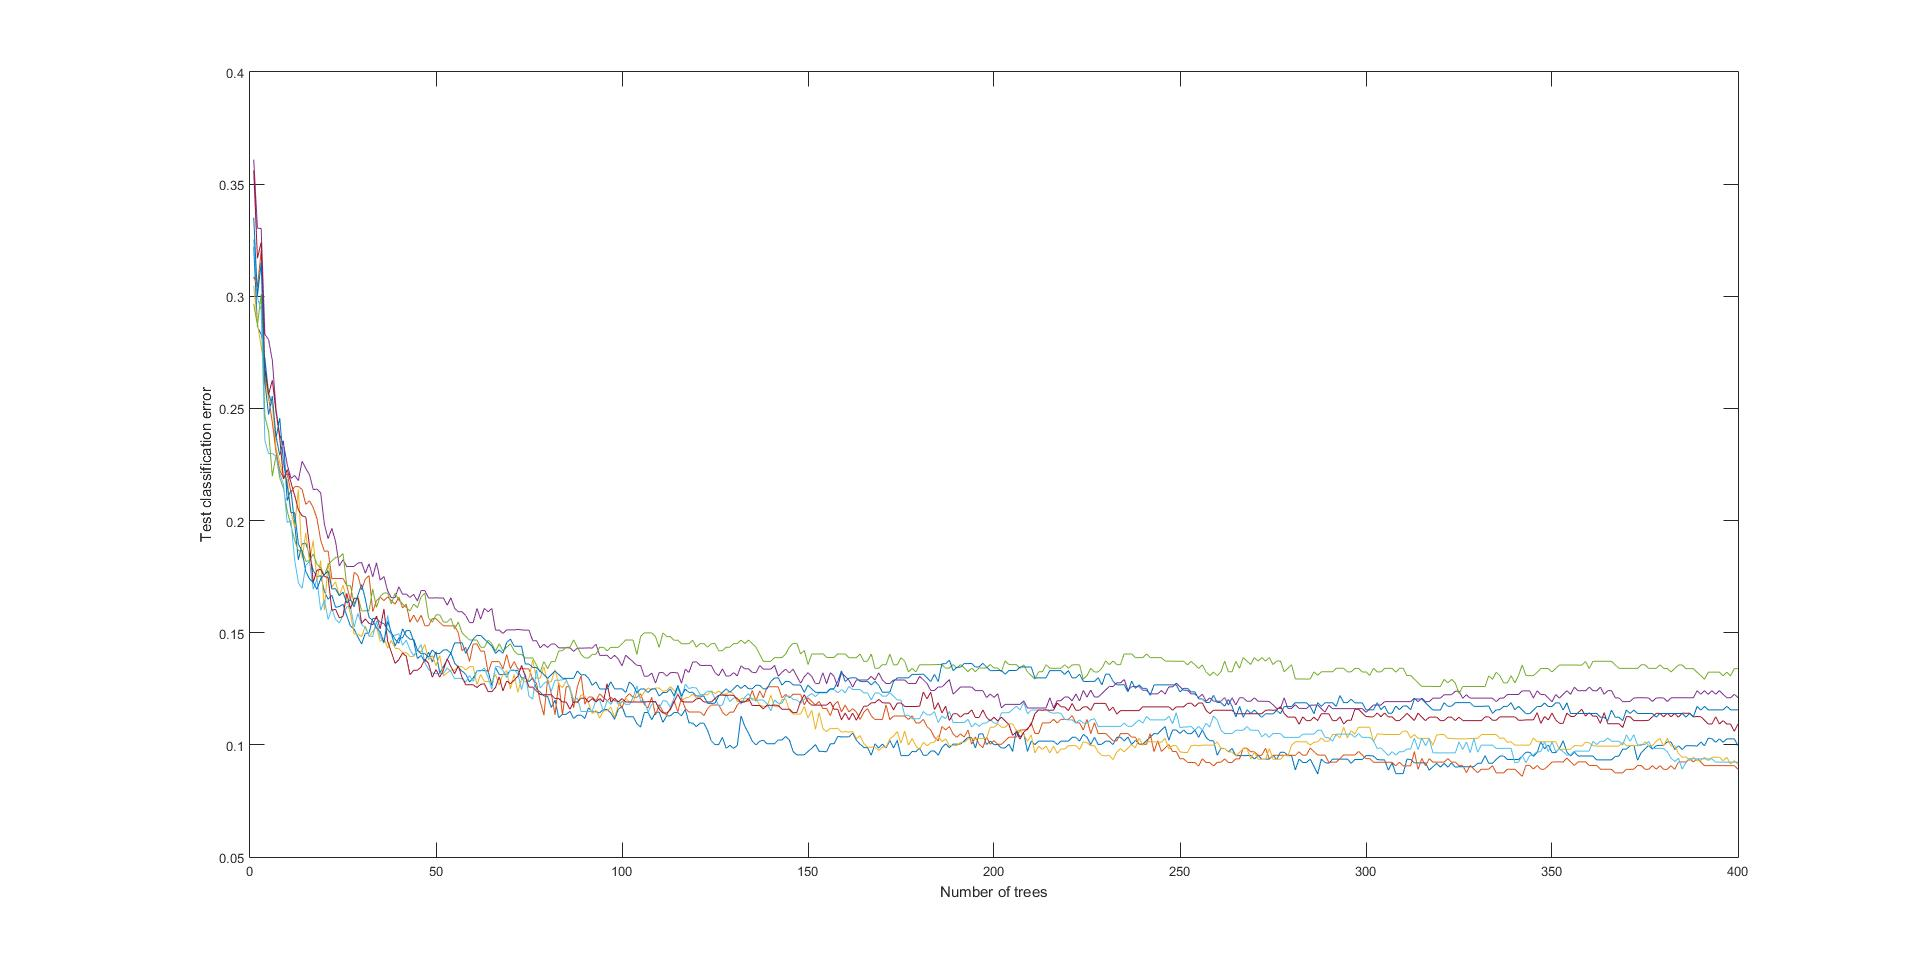
\includegraphics[scale=0.25]{logitboost.jpg}
\end{center}
\subsubsection{Kernel SVM}
\subsection{Classification on Image Features}
\subsubsection{Grey-scale Images}
We first converted the profile images data into R, G, B and Grey-scale images. 
\subsubsection{Face Detection with Viola-Jones Algorithm}
We extracted all the faces. We used matlab built-in Viola-Jones algorithm to do face detection on RGB images, which detected faces on 72\% of the profile pictures. All the following classifications over images were based on the faces detected. Later when ensemble, we only used samples with detected faces. For those samples without faces in them, we just set the output of the classifier as 0 (the output of the classifier is either positive or negative for male or female).
\subsubsection{Logistic Regression with Eigen Faces}
After extracted faces, we did PCA over grey-scale images, the visualization of the top principal components are shown in figure below. We put top PCs into logistic regression classifier and it yielded 60+\% accuracy. \\
\begin{center}
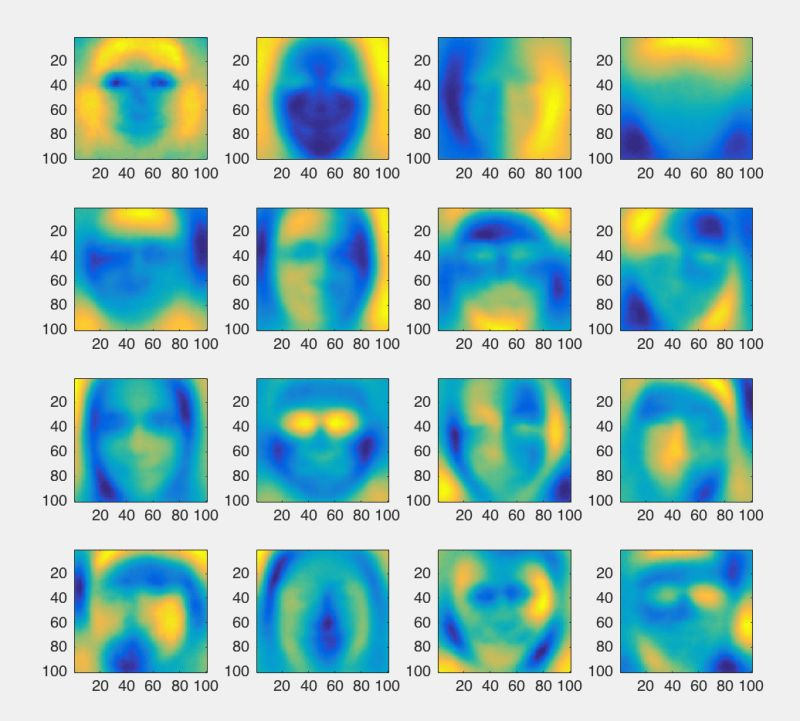
\includegraphics[scale=0.5]{pca_faces}
\end{center}
\subsubsection{HOG Features, Gaussian Pyramid, Eyes and Nose}
We used Viola-Jones algorithm to detect and crop eyes and nose. After that, we extracted Gaussian Pyramid HOG features into 7020 feature vector. Classifying the features with logistic regression yielded 82\% accuracy by itself on 72\% detected faces. The ensemble with this classifier produced 91.9\% over all accuracy on the test set. 
\subsubsection{SVM on PCA-ed HOG Features}
We then replaced the logistic regression classifier with a more powerful RBF kernel SVM. The accuracy on detected faces was improved up to 83\%. The ensemble with this classifier got 92.3\% accuracy on the test set.  Then we did PCA (1500 PCs) on HOG features to reduce the dimensionality and the size of SVM model. The accuracy of the single model with improved to 84\%. However, the ensemble with this classifier dropped to 92.14\% accuracy on the test set. 
\subsubsection{SVM on PCA-ed Dense LBP Features}
LBP works complementary with HOG features, we extracted spatial pyramid LBP features (15871 features) on detected faces. And trained a SVM classifier over 2000 principal components of the LBP features. This model achieved 85\% accuracy on detected faces. We integrated this model to the ensemble yielded our highest accuracy on the leaderboard of 92.42\% on test set.
\subsubsection{Bagging Logistic Regression on Raw HOG Features}
To meet the time and space constraints of the competition, we dropped LBP model and and replaced the SVM model with bagging logistic regression. Because the basis of PCs took 130Mb, which was too large for 50m space constraint, we didn't do PCA in the final submission either. Instead we used a bagging logistic regression with 6 logistic regression  models. The final model produced 91.04\% accuracy on validation set.
\subsubsection{Auto-encoder}
\subsection{Ensemble Methods}
\subsubsection{Stacking}
We used stacking to ensemble our models to achieve better over all performance than any of the single models. First, we used 80\% of the training data to train all the single models including logistic regression, neural network, logitboost with feature selection, kernel SVM with feature selection, kernel SVM with normalization, SVM over PCA-ed HOG, SVM over PCA-ed LBP. And then, use those models to generate predictions (scores) for the rest 20\% data. Training a logistic regression model using the 20\% scores with labels yields a ensemble classifier. Finally, we use all the training data to re-train all the single models. Along with the ensemble classifier, we got our final model. Our full model yielded 92.42\% prediction accuracy on the leaderboard over test set. For the final submission, due to the space and time constraints, we dropped the LBP model and replaced the SVM over PCA-ed HOG with bagging logistic regression over raw HOG features. This final submission yielded 91.04\% prediction accuracy on validation set, ranked 6th out of 50 teams.
\subsubsection{Normalization}
When ensemble all the models, we notices that normalization actually works. For the images, we first trained logistic regression on raw gaussian pyramid HOG features (faces, eyes and nose), which yielded 82\% accuracy on detected faces by itself. Later, we figured SVM works better by experiment (84\%). However, when we ensemble the new model, it actually produced lower accuracy. We then found that the scores ranges produced by logistic regression and SVM were actually different. This may cause unbalanced weights across models. We then normalized all the scores with a sigmoid function with mean 0 and variance 2. This produced higher overall accuracy (92.3\%). Tweaking the sigmoid function parameters for each model may produce a little bit higher accuracy but we didn't get enough time for that.
\subsubsection{Cascaded Ensembling}


